% Преамбула TeX-файла

% 1. Стиль и язык
\documentclass[utf8x]{G7-32} % Стиль (по умолчанию будет 14pt)
\usepackage[T2A]{fontenc}
\usepackage[russian]{babel}
\usepackage{setspace,lipsum}
\PassOptionsToPackage{shorthands=off}{babel}
\usepackage{bm}

\usepackage{mathtools}
\usepackage{caption}
\usepackage{subcaption}
\usepackage{setspace}
\usepackage{pgfplots}
\pgfplotsset{compat=newest}
\usepackage{filecontents}
\usepackage{animate}
\usepackage{graphics}
\usepackage{color}
\usepackage{fancyhdr}
\usepackage{lipsum}

\newcommand\blfootnote[1]{%
  \begingroup
  \renewcommand\thefootnote{}\footnote{#1}%
  \addtocounter{footnote}{-1}%
  \endgroup
}
\def\alert#1{\textcolor{red}{#1}}

\usepgfplotslibrary{dateplot}


% Остальные стандартные настройки убраны в preamble.inc.tex.
\sloppy

% Настройки стиля ГОСТ 7-32
% Для начала определяем, хотим мы или нет, чтобы рисунки и таблицы нумеровались в пределах раздела, или нам нужна сквозная нумерация.
\EqInChapter % формулы будут нумероваться в пределах раздела
\TableInChapter % таблицы будут нумероваться в пределах раздела
\PicInChapter % рисунки будут нумероваться в пределах раздела

% Добавляем гипертекстовое оглавление в PDF
\usepackage[
bookmarks=true, colorlinks=true, unicode=true,
urlcolor=black,linkcolor=black, anchorcolor=black,
citecolor=black, menucolor=black, filecolor=black,
]{hyperref}

% Изменение начертания шрифта --- после чего выглядит таймсоподобно.
% apt-get install scalable-cyrfonts-tex

\IfFileExists{cyrtimes.sty}
    {
        \usepackage{cyrtimespatched}
    }
    {
        % А если Times нету, то будет CM...
    }

\usepackage{graphicx}   % Пакет для включения рисунков

% С такими оно полями оно работает по-умолчанию:
% \RequirePackage[left=20mm,right=10mm,top=20mm,bottom=20mm,headsep=0pt]{geometry}
% Если вас тошнит от поля в 10мм --- увеличивайте до 20-ти, ну и про переплёт не забывайте:
\geometry{right=20mm}
\geometry{left=30mm}


% Пакет Tikz
\usepackage{tikz}
\usetikzlibrary{arrows,positioning,shadows,shapes,patterns,spy,calc}
\usetikzlibrary{shapes.geometric}
\usetikzlibrary{decorations.markings}
%\usetikzlibrary{shapes.geometric,arrows.meta}


% Произвольная нумерация списков.
\usepackage{enumerate}

% ячейки в несколько строчек
\usepackage{multirow}

% itemize внутри tabular
\usepackage{paralist,array}


% Настройки листингов.
% 8 Листинги

\usepackage{listings}

% Значения по умолчанию
\lstset{
  basicstyle= \footnotesize,
  breakatwhitespace=true,% разрыв строк только на whitespacce
  breaklines=true,       % переносить длинные строки
%   captionpos=b,          % подписи снизу -- вроде не надо
  inputencoding=koi8-r,
  numbers=left,          % нумерация слева
  numberstyle=\footnotesize,
  showspaces=false,      % показывать пробелы подчеркиваниями -- идиотизм 70-х годов
  showstringspaces=false,
  showtabs=false,        % и табы тоже
  stepnumber=1,
  tabsize=4,              % кому нужны табы по 8 символов?
  frame=single
}

% Стиль для псевдокода: строчки обычно короткие, поэтому размер шрифта побольше
\lstdefinestyle{pseudocode}{
  basicstyle=\small,
  keywordstyle=\color{black}\bfseries\underbar,
  language=Pseudocode,
  numberstyle=\footnotesize,
  commentstyle=\footnotesize\it
}

% Стиль для обычного кода: маленький шрифт
\lstdefinestyle{realcode}{
  basicstyle=\scriptsize,
  numberstyle=\footnotesize
}

% Стиль для коротких кусков обычного кода: средний шрифт
\lstdefinestyle{simplecode}{
  basicstyle=\footnotesize,
  numberstyle=\footnotesize
}

% Стиль для BNF
\lstdefinestyle{grammar}{
  basicstyle=\footnotesize,
  numberstyle=\footnotesize,
  stringstyle=\bfseries\ttfamily,
  language=BNF
}

% Определим свой язык для написания псевдокодов на основе Python
\lstdefinelanguage[]{Pseudocode}[]{Python}{
  morekeywords={each,empty,wait,do},% ключевые слова добавлять сюда
  morecomment=[s]{\{}{\}},% комменты {а-ля Pascal} смотрятся нагляднее
  literate=% а сюда добавлять операторы, которые хотите отображать как мат. символы
    {->}{\ensuremath{$\rightarrow$}~}2%
    {<-}{\ensuremath{$\leftarrow$}~}2%
    {:=}{\ensuremath{$\leftarrow$}~}2%
    {<--}{\ensuremath{$\Longleftarrow$}~}2%
}[keywords,comments]

% Свой язык для задания грамматик в BNF
\lstdefinelanguage[]{BNF}[]{}{
  morekeywords={},
  morecomment=[s]{@}{@},
  morestring=[b]",%
  literate=%
    {->}{\ensuremath{$\rightarrow$}~}2%
    {*}{\ensuremath{$^*$}~}2%
    {+}{\ensuremath{$^+$}~}2%
    {|}{\ensuremath{$|$}~}2%
}[keywords,comments,strings]

% Подписи к листингам на русском языке.
\renewcommand\lstlistingname{\cyr\CYRL\cyri\cyrs\cyrt\cyri\cyrn\cyrg}
\renewcommand\lstlistlistingname{\cyr\CYRL\cyri\cyrs\cyrt\cyri\cyrn\cyrg\cyri}

\definecolor{codegreen}{rgb}{0,0.6,0}
\definecolor{codegray}{rgb}{0.5,0.5,0.5}
\definecolor{codepurple}{rgb}{0.58,0,0.82}
\definecolor{backcolour}{rgb}{0.95,0.95,0.92}

\lstdefinestyle{mystyle}{
    backgroundcolor=\color{backcolour},   
    commentstyle=\color{codegreen},
    keywordstyle=\color{magenta},
    numberstyle=\tiny\color{codegray},
    stringstyle=\color{codepurple},
    basicstyle=\ttfamily\footnotesize,
    breakatwhitespace=false,         
    breaklines=true,                 
    captionpos=b,                    
    keepspaces=true,                 
    numbers=left,                    
    numbersep=5pt,                  
    showspaces=false,                
    showstringspaces=false,
    showtabs=false,                  
    tabsize=2
}

\lstset{style=mystyle}


% Полезные макросы листингов.
% Любимые команды
\newcommand{\Code}[1]{\textbf{#1}}



\begin{document}

\thispagestyle{empty}
\pagestyle{fancy}
\fancyhf{}
\fancyhead[C]{\thepage}
\renewcommand{\headrulewidth}{0pt}
\newgeometry{top=2cm,bottom=3cm,left=3cm,right=1cm}
{
\singlespacing
\begin{center}

ФГБУН <<Институт системного программирования им. В.П. Иванникова>>
\medskip
\hrule
\medskip
\end{center}

\vspace{20mm}
\begin{flushright}
На правах рукописи

%{\sl УДК 519.713.3}
\end{flushright}

\vspace{25mm}
\begin{center}
{\large Рязанов Даниил Александрович}
\end{center}

\vspace{5mm}
\begin{center}
{\bf \large Бигармонические аттракторы внутренних волн 
\par}

\vspace{10mm}
{
01.02.05~--- Механика жидкости газа и плазмы
}

%\parbox{0.88\textwidth}{
%Специальность 05.13.17~---
%Теоретические основы информатики
%}
%\parbox{0.88\textwidth}{
%\vspace{5mm}
%Специальность 05.13.19~---
%Методы и системы защиты информации,
%}
%информационная безопасность

%\begin{tabular}{r c l}
%Специальность 05.13.17& --- &Теоретические основы информатики\\[3mm]
%Специальность 05.13.19& --- &\parbox[t]{10cm}{Методы и системы защиты информации,\\ \centering информационная безопасность}
%\end{tabular}



\vspace{10mm}

{\bf \large Автореферат
\par}

\vspace{10mm}

 диссертации на соискание ученой степени кандидата физико-математических наук
\end{center}

% \vspace{16mm}
% \begin{flushright}
% Научный руководитель:\\[2mm]
% д.ф.-м.н., \\
% Веденеев~В.\,В.\\

% \end{flushright}

\vfill
\begin{center}
{Москва -- 2021}
\end{center}
}
\newpage
\restoregeometry

\newpage
\pagestyle{empty}
\begin{spacing}{1.2}
\pagestyle{empty}
\begin{flushleft}
  Работа выполнена в ИСП им. В.П. Иванникова РАН
\end{flushleft}
\pagestyle{empty}
\begin{flushleft}
\begin{tabular}{p{5.8cm} p{10.5cm}}
    Научный руководитель: & к. ф.-м. н. Сибгатуллин Ильяс Наилевич, старший научный сотрудник, Института океанологии им. П.П. Ширшова РАН  \\

    \\

    Официальные оппоненты: &  д. ф.-м. н., Петров Александр Георгиевич, ведущий научный сотрудник Института проблем механики имени А.~Ю.~Ишлинского РАН. \\
  

    \\

    & к. ф.-м. н., доцент, Нуриев Артем Наилевич, научный сотрудник Казанского федерального университета (г. Казань).
    
    \\

    Ведущая организация: & Федеральное государственное бюджетное учреждение науки 
    Институт гидродинамики им. М.А. Лаврентьева Сибирского отделения Российской академии наук (г. Новосибирск). 
    
\end{tabular}
\end{flushleft}

\begin{flushleft}
    Защита состоится 15 октября 2021 г. в 11:00 часов на заседании диссертационного совета Д 002.024.01, созданного на базе ИПМ им. М.В. Келдыша РАН, 125047, Москва, Миусская пл., д.4

    \setlength{\parskip}{1em}

    С диссертацией можно ознакомиться в библиотеке и на сайте ИПМ им. М.В. Келдыша РАН http://keldysh.ru 

    \setlength{\parskip}{1em}
    \vspace{1cm}
    Автореферат разослан «\underline{\hspace{1cm}}» \underline{\hspace{4cm}} 2021 г.    
\end{flushleft}
\vspace{2cm}
\setlength{\parskip}{1em}
\begin{flushleft}
    \begin{tabular}{p{10cm} p{5cm}}

        Учёный секретарь диссертационного совета \\ к.ф.-м.н.  
    & М.А. Корнилина  
        
    \end{tabular}
\end{flushleft}
\end{spacing}
\newpage

\setcounter{page}{3}
\pagestyle{fancy}
\setcounter{secnumdepth}{-1}

\section{Общая характеристика работы}

% Важной задачей изучения аттракторов внутренних волн с помощью численных методов является обеспечение возможности проводить численные эксперименты с геометрией, приближенной к геометрии реального дна океана. Выполнение этой задачи ускорило и удешевило бы процесс непостредственного поиска аттракторов внутренних волн в океане, и изучение влияния аттркаторов на турбулентные режимы. Метод спектральных элементов, который обеспечивает достаточную точность воспроизведения результатов эксперимента, ограничен в своей реализации сложностью геометрии расчетной области. В свою очередь, метод конечного объема позволяет работать со сложной геометрией, которая способна имитировать поверхность океанического дна, но стандартные реализации не обладают достаточной точностью. Кроме того, монохроматический источника возмущений может не описывать реальные внешние воздействия. Зачастую, при моделировании явлений, связанных с образованием аттракторов в реальных условиях, необходимо учитывать несколько приливных воздействий и изменение стратификации.

\paragraph{Актуальность работы.}

Внутренние волны из-за особенностей своего распространения имеют возможность фокусироваться. Многократное отражение от наклонных поверхностей, которые являются частью рельефа морского дна, ведет к накоплению кинетической энергии и интенсификации движения стратифицированной жидкости. Такое явления называются волновым аттрактором. Волновые аттракторы в океанах из-за значительных запасов кинетической энергии должны влиять на необратимое перемешивание стратифицированной жидкости, седиментацию примесей, поведение живых организмов. 

Волновые структуры, называемые волновыми аттракторами, в явном виде воспроизводятся на лабораторных установках, но их моделирование в условиях приближенных к природным имеет ряд значительных сложностей. Прежде всего из-за перехода к турбулентному режиму, большого количества источников внешних возмущений(вместо одного при лабораторных условиях), сложной геометрии морского дна и нелинейный профиль солености. Эти особенности течения в условиях приближенных к реальным может исказить четкую структуру волнового аттрактора, наблюдаемую в лабораторных условиях. 

В этой работе рассматривается периодические воздействия на стратифицированную жидкость с двумя частотами, которые соответствуют двум различным конфигурациям волновых аттракторов. Выясняется возможность существования аттракторов при бигармоническом воздействии на стратифицированную жидкость и способы взаимодействия внутренних волн различных частот. 

Решение задач моделирования аттракторов внутренних волн в условиях сложных геометриях, порождаемых источниками возмущения различной частоты и амплитуды поможет описать течения, возникающие в результате многократных отражений внутренних волн от рельефа дна океана. Результаты моделирования позволят дать первичную оценку влияния аттракторов на перемешивание в стратифицированной жидкости, на процессы седиментации различных веществ, на эрозию конструкций и рельефа в областях повышенной интенсивности движения жидкости, на паттерны поведения различных форм жизни в условиях сосуществования с аттрактором внутренних волн. Результаты работы представляют собой интерес для приложений в океанологии, экологии, биологии, астрофизики и вращающихся технических систем. 

\paragraph{Цель работы} -- изучение явления бигармонического аттрактора, которое возникает при воздействии на стратифицированную жидкость двухчастотным волнопродуктором.  
С этой целью были поставлены следующие \textbf{задачи}:

\begin{itemize}

  \item Нахождение интервала частот внешних воздействий, при которых возникает аттрактор внутренних волн.
  
  % Изучение интервалов частот внешних воздействий и других параметров, при которых происходит аккумуляция волновой энергии, в частности волновых аттракторов.

%    \item Нахождение частотных параметров приводящих к образованию аттракторов в резервуаре.
    
  % \item Обзор существующих методов моделирования аттракторов внутренних волн. Выявление их достоинств и недостатков.
    
  \item Реализация численных экспериментов с помощью двух подходов: спектрально-элементного и конечно-объемного.

  \item Разработка новой программы для моделирования аттракторов внутренних волн на основе квазигидродинамического подхода.
    
  \item Верификация результатов численного моделирования.

  \item Описание особенностей волновых режимов при бигармоническом воздействии и значительно отличающихся частотах воздействия и малых амплитудах.

  \item Описание особенностей волновых режимов при бигармоническом воздействии, близких частотах воздействия и малых амплитудах.
    
  \item Описание особенностей нелинейных волновых режимов при бигармоническом воздействии и близких частотах воздействия.

  \item Сравнение динамики средней кинетической энергии и пульсации кинетической энергии для монохроматического режима и различных бигармонических режимов.
    

    
\end{itemize}

\paragraph{Методы решения поставленных задач}

Для решения поставленных задач были использованы методы математического моделирования механики сплошных сред, такие как метод спектральных элементов и метод конечного объема. Для предсказания формы аттрактора внутренних волн использовался метод трассировки лучей. Для анализа данных использовался метод построения частотно-временных диаграмм при помощи быстрого преобразования Фурье.

\paragraph{Научная новизна работы} выражается в конкретных результатах:
\begin{enumerate}[1.]
  \item Получены аналитические выражения для границ частотного интервала существования аттракторов внутренних волн.% конфигурации (1,1). 
    
  \item Получена геометрия течения, которая возникает в трапециевидном резервуаре, наполненном стратифицированной жидкостью при воздействии на жидкость внешними возмущениями с двумя различными частотами. 
    
  \item Проведён анализ результатов моделирования аттрактора внутренних волн при бигармоническом воздействии, полученных с помощью метода спектральных элементов. Для различных комбинаций возмущающих частот построен спектр, частотно-временная диаграмма и зависимость средней кинетической энергии от времени. 
    
  \item Реализован квазигидродинамический подход на базе метода конечного элемента. Проведено сопоставление результатов моделирования методом конечных объемов и методом спектральных элементов.
\end{enumerate}

\paragraph{Достоверность результатов}

Достоверность полученных результатов гарантируется строгой математической постановкой, верификацией и валидацией разработанного алгоритма для решения поставленной задачи.

% \paragraph{Объектом исследования} являются волновые режимы возникающие %в естественных условиях 
% при двух источниках внешних воздействий на стратифицированную жидкость в трапециевидном резервуаре.

% %Приложения включают в себя задачи океанологии, астрофизики и технических вращающихся систем при периодических воздействиях. 

% %\paragraph{В исследовании использованы следующие методы:}
% \begin{itemize}
%   \item [    В исследовании использованы \textbf{
% методы:}]
%   \item методы численного моделирования конечного объема;
%   \item метод спектральных элементов;
%   \item метод трассировки лучей;
%   \item Фурье анализ полученных результатов, в том числе по скользящему окну;
%   \item разложение по эмпирическим модам;
% \end{itemize}

% % В работе рассматриваются резервуары в форме трапеций различных конфигураций, заполненных стратифицированной жидкостью. Одна из стенок резервуара представляет собой волнопродуктор, который порождает внутренние волны в стратифицированной среде. Результаты разработки предоставляют возможность проводить моделирование аттракторов внутренних волн в условиях сложной геометрии и неортогональных сетках. 
 
\paragraph{Практическая значимость} 

Ранее эксперименты по исследованию бигармонических аттракторов, как численные так и натурные, не проводились. Теоретически, бигармонический аттрактор представляет собой новую устойчивую структуру, которая образуется в стратифицированной жидкости при воздействии на нее периодическим двухчастотным возмущением.

Положения и выводы диссертационного исследования могут быть использованы для подбора параметров  волнового аттрактора в лабораторных условиях или при численном моделировании. Среди возможных приложений результатов работы — задачи моделирования аттракторов внутренних волн на сложных геометриях, задачи моделирования течений со сложным спектром частотных воздействий на стратифицированную жидкость. Работа является первым шагом к моделированию течений, возникающих в условиях, приближенных к реальным океаническим, что позволит выяснить форму и вид природных аттракторов внутренних волн. Комбинация методов конечного объёма и квазигидродинамических уравнений позволила добиться существенного улучшения в точности моделирования и дала инструмент к  усложнению геометрии расчётной области. Разработанная программа может быть применена не только к задачам моделирования аттрактора, но и к другим задачам гидродинамики с дозвуковыми и трансзвуковыми скоростями.

\paragraph{На защиту выносятся следующие положения}
\begin{itemize}

  \item Найдены аналитические выражения для границ диапазонов частот колебаний волнопродуктора, которые способны порождать аттракторы.

  \item Показано, что при значительном отличии частот внешних воздействий и малых амплитудах воздействий волновой режим представляет собой совокупность независимо существующих волновых аттракторов.

  \item Показано, что при близких частотах внешних воздействий и малых амплитудах возникает режим с биениями, характерной особенностью которых является малая амплитуда пульсаций на убывающем склоне огибающей.

  \item Показано, что при близких частотах внешних воздействий и средних амплитудах возникают биения, на одном цикле которых успевает происходить переход к турбулентности через триадные резонансы, и реламинаризация.
    
  \item Обнаружено наличие фазового сдвига между биениями на волнопродукторе и биениями средней кинетической энергии во всем объеме.
    
%   \item 
%     Сравнение динамики средней кинетической энергии и пульсации кинетической энергии для монохроматического режима и различных бигармонических режимов указывает на то, что на убывающем склоне огибающей большая доля кинетической энергии переходит в бегущие волны по сравнению с возрастающей фазой.

  \item Разработана и верифицирована новая программа для моделирования аттракторов внутренних волн и в целом динамики стратифицированных сред.
    
%  \item Реализация численных экспериментов с помощью двух подходов: спектрально-элементного и конечно-объемного.

%  \item Проведена верификация результатов численного моделирования.
%    Проведение численных экспериментов различными методами.
    
%  \item Количественный анализ результатов численных экспериментов. 
    
%  \item Верификация разработанной программы.
    
\end{itemize}

\paragraph{Личный вклад автора}

Исследования, результаты которых выносятся на защиту, были получены лично соискателем. Соискатель аналитически нашел диапазон частот внешнего воздействия при которых образуется аттрактор внутренних волн. Соискатель подобрал параметры эксперимента, провел расчеты и проанализировал полученные данные. Также принимал непосредственное участие в разработке реализации квазигидродинамического подхода на базе открытого программного комплекса OpenFOAM. Научный руководитель И. Н. Сибгатуллин поставил первоначальную задачу и участвовал в обсуждении результатов. 

\paragraph{Апробация работы}

Материалы диссертации представлялись на различных конференциях, семинарах, как российских так и международных:


\begin{itemize}
  \item Открытая международная конференция ИСП РАН им. В.П.Иванникова. 5-6 декабря 2019 г, г. Москва Главное здание Российской академии наук (устный доклад).
  \item Международная конференция «Суперкомпьютерные технологии математического моделирования» (СКТеММ’19), 19-21 июня 2019, г. Москва (устный доклад).
  \item 13th OpenFOAM Workshop, Shanghai, China, Китай, 24-29 июня 2018 (устный доклад).
  \item XXIII международная конференция «Нелинейные задачи теории гидродинамической устойчивости и турбулентность». 25 февраля - 4 марта 2018, Московская область, г. Звенигород (стендовый доклад).
  \item Рязанов Д.А. Открытая конференция ИСП РАН им. В.П. Иванникова. 30 ноября - 1 декабря 2017 г. Москва главное здание Российской академии наук (стендовый доклад).
\end{itemize}

\paragraph{Публикации}

По результатам диссертации опубликовано 12 научных работ, входящих в базы данных и системы цитирования РИНЦ, Scopus, Web of Science, 2 из них входят в Перечень рецензируемых научных изданий, рекомендованных Высшей аттестационной комиссией. Зарегистрирована программа для ЭВМ. Автор также принимал участие в проекте связанном с темой диссертации грант РНФ № 19-11-00169.

\paragraph{Структура и объем диссертации}

Диссертация состоит из введения, обзора литературы, трех глав, заключения и списка литературы. Текст работы содержит 106 печатных страниц, 59 рисунков и 6 таблиц. Список литературы включает в себя 90 наименований. 


















































\renewcommand\thefigure{\arabic{figure}}

\section*{Содержание работы}

Работа состоит из \textbf{введения}, где обозначены цели и задачи, сформулирована теоретическая значимость, практическая применимость проведенного исследования.  Также описаны методы используемые в работе, обозначен личный вклад автора, перечислены выносимые на защиту положения.

\textbf{Первая глава} посвящена обзору существующих исследований в области аттракторов внутренних волн и стратифицированной жидкости. Обзор литературы содержит в себе историю развития теории внутренних волн и описание основных событий, которые заострили внимание научной общественности на этом явлении. Дано понятие о возникновении внутренних волн в непрерывно стратифицированной жидкости, их свойства. Приведена классическая математическая модель описания динамики стратифицированной жидкости, включающая в себя уравнение движения
\begin{equation*}
 \large \frac{\partial \vec U}{\partial t} + (\vec U \cdot \nabla) \vec U = - \frac{1}{\rho_m} \nabla \hat p + \nu \Delta \vec U  + \vec f,
 \label{eq:momClassic}
\end{equation*}

\noindent уравнение переноса соли $s$
\begin{equation*}
 \large \frac{\partial \rho_s}{\partial t} + \vec U \cdot \nabla \rho_s  = \nabla \cdot \frac{\nu}{Sc} \left ( \nabla \rho_s \right ),
 \label{eq:transClassic}
\end{equation*}

\noindent и уравнение неразрывности
\begin{equation*}
 \large \nabla \cdot \vec U  = 0.
 \label{eq:contClassic}
\end{equation*}

\noindent дисперсионное соотношение для внутренних волн 
\begin{equation}
    \frac{\omega}{N} = \pm sin \theta.
    \label{eq:dispersion}
\end{equation}
В этой главе дается определение аттракторов внутренних волн, как геометрической зоны притяжения лучей направленных вдоль групповой скорости внутренних волн. Для фокусировки внутренних волн в лабораторных и численных экспериментах используется трапециевидный резервуар (Рис. \ref{fig:dominleft}), который заполняется линейно стратифицированной жидкостью.  Благодаря свойству фокусировки волновые лучи сходятся к паралелелограму и циркулируют по его сторонам (рис. \ref{fig:RayTr}). Физически аттрактор внутренних волн представляет собой зону интенсивного движения жидкости (рис. \ref{fig:attractorRes}).

\begin{figure}[!ht]
        \centering
          \begin{tikzpicture}[scale=1.5, z={(-.707,-.5)}]
            \draw (0,0,0) -- (6,0,0) -- (4,4,0)--(0,4,0) --cycle;
            \draw (0,0,0)     -- (6,0,0)   -- (4,4,0)   -- (0,4,0)    -- cycle;
            \draw[style = dashed] (2.7,4,0)   -- (0,1.8,0) -- (2.2,0,0) -- (5,2.1,0)-- cycle;
            %\draw[style = dashed] (0,0.985,0) -- (3.3,4,0) -- (4.5,3,0) -- (1.1,0,0)  -- cycle;

            \draw[<->] (-0.1,0) --node[above,rotate=90] {$H = 40$ cm} (-0.1,4);
            \draw[<->] (0,-0.1,0) --node[below,] {$L_2 = 60$ cm} (6,-0.1,0);
            \draw[<->] (0,4.1,0) --node[above,] {$L_1 = 40$ cm} (4,4.1,0);

            \draw[color=red] (3.0,0)--(3.0,4.0);
            
            \draw (3.15,0) node[above] {$A$};
            \draw (3.15,4.0) node[below] {$B$};

            \draw[thick,->] (4.95,3.5,0) -- (5.95,3.5,0) node[anchor=north east]{$x$};
            \draw[thick,->] (4.95,3.5,0) -- (4.95,4.5,0) node[anchor=north west]{$z$};
            \draw[thick,->] (5.3,3,0) -- (5.3,2,0) node[anchor=west]{$\vec{g}$};
          \end{tikzpicture}
          \caption{Вычислительная область для аттракторов внутренних волн, красным показана линия пробы, пунктиром показана предполагаемая форма аттрактора}
          \label{fig:dominleft}
\end{figure}

\begin{figure}[h!]
    \centering
    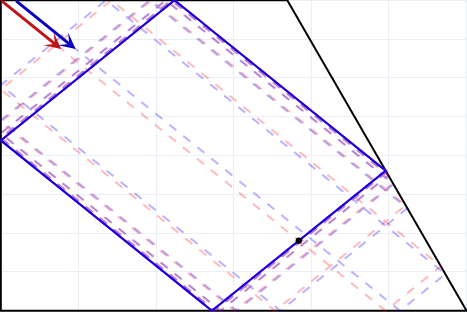
\includegraphics[scale=1.1]{../Figs/RayTracing1.png}
    \caption{Результат многократного отражения двух параллельных лучей внутренних волн}
    \label{fig:RayTr}
\end{figure}

\begin{figure}[!ht]
    \centering
        \begin{tikzpicture}[scale=4.64, z={(-.707,-.5)}]
          \node[anchor=south west,inner sep=0] at (0,0) {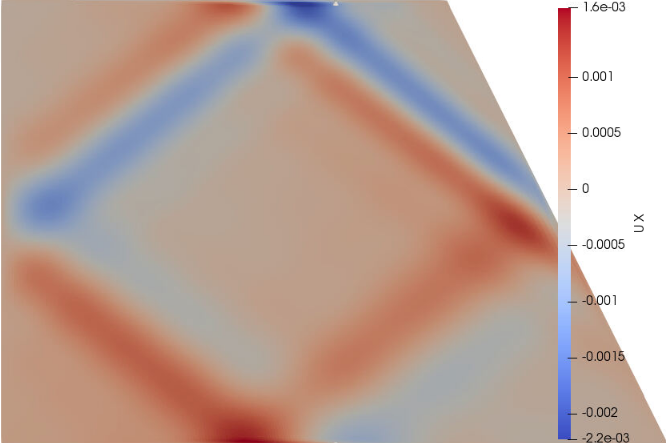
\includegraphics[width=0.87\textwidth]{../Figs/Attr200s.png}};
          \draw[thick,style = dashed] (1.5, 0, 0) -- (1.5, 2, 0);
        \end{tikzpicture}
    \caption{Поле горизонтальной компоненты скорости, пунктиром показана линия пробы}
    \label{fig:attractorRes}
\end{figure}

Во \textbf{второй главе} обозреваются методы исследования аттракторов внутренних волн. Прежде всего это предсказание траекторий групповых скоростей с помощью метода трассировки лучей -- простого и мощного инструмента моделирования аттракторов внутренних волн. Суть его в геометрическом вычислении зоны притяжения волновых лучей после множественных отражений (рис. \ref{fig:RayTr}). Метод позволяет предсказывать форму аттрактора внутренних волн, но не позволяет получить значение гидродинамических полей. Этот метод полезен для понимания того какие частоты колебаний волнопродуктора приводят к формированию аттрактора внутренних волн, а какие не приводят.

Раздел с экспериментальными исследованиями посвящён лабораторным установкам и способам получения внутренних волн в лабораторных условиях. Упоминаются коллективы во Франции и России, которые занимаются проблемой внутренних волн.

В следующем разделе обозреваются методы численного моделирования аттракторов внутренних волн. Дана характеристика методу спектральных элементов для моделирования аттракторов внутренних волн как очень мощный инструмент высокого порядка. Однако, метод спектральных элементов очень чувствителен к вычислительной сетке и геометрии. Метод не подходит для моделирования аттракторов внутренних волн в естественных условиях сложной топологии океанического дна или при наличии примесей описываемых частицами в воде. Этот метод дает результаты значений гидродинамических полей давления и скорости очень близко к результатам экспериментальных исследований. Метод спектральных элементов используется как эталон в этой работе.

Альтернативный метод -- метод конечных объемов. Позволяет проводить численные эксперименты в условиях приближенных к реальным, включая сложную геометрию океанического дна и осаждение примесей. Однако, его реализация на одной из самых популярных платформ не демонстрирует сеточной сходимости и количественного соответствия методу спектральных элементов. Метод конечных объемов и его реализация в пакете OpenFOAM не позволяет достичь той точности, что гарантирует метод спектральных элементов. Стандартные средства популярных инструментов моделирования несжимаемых течений не могут количественно воспроизвести эффекты множественной фокусировки внутренних волн (рис. \ref{fig:meshAttr300PISO}).

\begin{figure}
    \centering
        \begin{tikzpicture}[scale = 1]
          \begin{axis}
             [scale only axis, grid=major,legend style={at={(0.3,1),font=\LARGE},anchor=north west}, ymin=-1.2*10^-3, ymax=1.7*10^-3, xmin=0.0,legend style={nodes={scale=0.5, transform shape}}, x post scale=1.5,xlabel={$y$}, ylabel={$U_x$}];

            \addplot[solid,thick, color=orange, dashed] table [x=y, y=U_0m, col sep=comma]
            {../CSV/U225x300A01w623corr31300_U.csv};
            \addplot[solid,thick, color=cyan] table [x=y, y=U_0m, col sep=comma]
            {../CSV/U300x450A01w623corr31300_U.csv};
            \addplot[solid,thick, color=blue] table [x=y, y=U_0m, col sep=comma]
            {../CSV/U450x600A01w623corr31300_U.csv};

            \legend{PISO 225x300,PISO 300x450,PISO 450x600}
          \end{axis}
          \begin{axis}
            [scale only axis, ymin=-1.2*10^-1, ymax=1.7*10^-1, xmin=0.0,  yticklabels={,,},xticklabels={,,},legend style={at={(0.3,0.8),font=\LARGE},anchor=north west},legend style={nodes={scale=0.5, transform shape}},x post scale=1.5];
            \addplot[solid,thick, color = red] table [x=Points:1, y=x_velocity, col sep=comma] {../CSV/NEK300s0.csv};
            \legend{NEK 5000}
          \end{axis}
        \end{tikzpicture}
    \caption{Сравнение горизонтальной компоненты скорости полученной при различных размерах расчетной сетки для алгоритма PISO с той же величиной полученной при помощи метода спектральных элементов.  Время = 300 с.}
    \label{fig:meshAttr300PISO}
\end{figure}

Подход на основе квазигидродинамических уравнений имеет простой вычислительный алгоритм, количественное совпадение результатов с результатами полученными при помощи метода спектральных элементов.

В главе также сказано о реализации квазигидродинамического подхода, верификации разработанного алгоритма и валидации на примере задачи формирования аттрактора внутренних волн сравниваются результаты работы алгоритма PISO и QHD. Результаты количественно сравнивались с эталонным решением, полученным при помощи метода спектральных элементов \ref{fig:meshAttr300}.

\begin{figure}
  \centering
      \begin{tikzpicture}[scale = 1]
        \begin{axis}
           [scale only axis, grid=major,legend style={at={(0.3,1),font=\LARGE},anchor=north west}, ymin=-1.2*10^-3, ymax=1.7*10^-3, xmin=0.0,legend style={nodes={scale=0.5, transform shape}}, x post scale=1.5,xlabel={$y$}, ylabel={$U_x$}];

          \addplot[solid,thick, color=red, dashed] table [x=y, y=U_0, col sep=comma]
          {../CSV/U225x300A01w623tau005t300_U.csv};
          \addplot[solid,thick, color=green] table [x=y, y=U_0, col sep=comma]
          {../CSV/U300x450A01w623tau005t300_U.csv};
          \addplot[solid,thick, color=blue] table [x=y, y=U_0, col sep=comma]
          {../CSV/U450x600A01w623tau005t300_U.csv};

          \legend{QHD 225x300,QHD 300x450,QHD 450x600}
        \end{axis}
        \begin{axis}
          [scale only axis, ymin=-1.2*10^-1, ymax=1.7*10^-1, xmin=0.0,  yticklabels={,,},xticklabels={,,},legend style={at={(0.3,0.8),font=\LARGE},anchor=north west},legend style={nodes={scale=0.5, transform shape}},x post scale=1.5];
          \addplot[solid,thick] table [x=Points:1, y=x_velocity, col sep=comma] {../CSV/NEK300s0.csv};
          \legend{NEK 5000}
        \end{axis}
      \end{tikzpicture}
  \caption{Сравнение горизонтальной компоненты скорости полученной при различных размерах расчетной сетки для алгоритма QHD с той же величиной полученной при помощи метода спектральных элементов.  Время = 300 с.}
  \label{fig:meshAttr300}
\end{figure}


\begin{figure}[hbt!]
    \centering
        
    \begin{tikzpicture}[scale = 1,spy using outlines={circle, magnification=6, connect spies}]
        \begin{axis}
            [scale only axis, xlabel=Линия пробы $m \cdot 10^{-3}$, ylabel=$U_x\;\; m/s \cdot 10^{-3}$, grid=major,legend style={at={(0,1),font=\LARGE},anchor=north west}, ymin=-0.8, ymax=0.8,xmin=0,xmax=20,legend style={nodes={scale=0.5, transform shape}}, x post scale=1.6]

            \addplot[solid,color=black,thick] table [x=Points:1, y=U, col sep=comma] {../CSV/NEK5000.csv};
            \addplot[solid,color=red,thick] table [x=Points:1, y=U, col sep=comma] {../CSV/QHD480x320.csv};
            \addplot[solid,color=green!60!black,thick] table [x=Points:1, y=U, col sep=comma] {../CSV/QHD240x160.csv};
            \addplot[solid,color=blue,thick] table [x=Points:1, y=U, col sep=comma] {../CSV/QHD240x1602tau.csv};
            \legend{NEK500,QHDFoam 480x320, QHDFoam 240x160, QHDFoam 240x160 $\tau \cdot 2$}

            \coordinate (spypoint) at (axis cs:14.7,0.7);
            \coordinate (magnifyglass) at (axis cs:15.5,-0.3);
        \end{axis}
        \spy [blue, size=4cm] on (spypoint) in node[fill=white] at (magnifyglass);
    \end{tikzpicture} 
    \caption{Количественное сравнение результатов моделирования}
    \label{fig:AdamsBashforthEulerNek3D}
\end{figure}

Анализ полученных результатов позволяет сделать следующие выводы:
\begin{itemize}
    \item На верификационной задаче о моделировании стационарного течения в скошенной каверне оба метода ведут себя одинаково адекватно, наблюдается сеточная сходимость численных результатов, что говорит об устойчивости методов на деформированных сетках.
    \item На задаче о моделировании формирования аттрактора гравитационных внутренних волн QHD алгоритм показывает результаты как количественно, так и качественно воспроизводящие это явление, как на малых, так и на больших временах. Алгоритм PISO воспроизводит явление лишь качественно и только на небольших временах.
    \item QHD алгоритм показывает сеточную сходимость и сходимость по регуляризационному настроечному параметру. PISO алгоритм не демонстрирует сеточной сходимости при сгущении пространственной сетки.
    \item QHD алгоритм, построенный на базе квазигидродинамических уравнений, не требует дополнительных коррекций вычисленных скоростей и давлений в отличие от алгоритма PISO.
    \item OpenFOAM реализация квазигидродинамического подхода показала более высокую производительность на многопроцессорной системе чем реализация алгоритма PISO.
\end{itemize}

Исходя из вышесказанного можно констатировать преимущества алгоритма QHD при моделировании аттракторов внутренних волн по сравнению со стандартными средствами, ранее реализованными в OpenFOAM на базе алгоритма PISO. 

%Раздел с численным моделированием аттракторов внутренних гравитационных волн содержит в себе результаты моделирования аттракторов с помощью метода спектральных элементов и контрольного объема алгоритмами PISO и QHD на базе открытого программного продукта OpenFOAM. Также в этом разделе обусловлен выбор частот для моделирования бигармонических колебаний, приведены результаты моделирования и анализ данных.

\textbf{Глава номер три} посвящена количественной оценке режимов течения в резервуаре с моно и бигармоническими воздействиями на стратифицированную жидкость. Для определения наиболее интересного диапазона параметров выполнено подробное исследование генерации аттракторов при монохроматическом возмущении, в результате чего определен частотный диапазон, в котором генерация аттракторов наиболее эффективна. Для моделирования бигармонического аттрактора внутренних волн используется специальное граничное условие для скорости на левой стенке трапецевидного резервуара:

$$U_z = A_1\cdot cos\left(\frac{\pi \cdot z}{L_1}\right)\cdot \omega_1 \cdot  sin(\omega_1 t) + A_2\cdot cos\left(\frac{\pi \cdot z}{L_1}\right)\cdot \omega_2 \cdot  sin(\omega_2 t).$$

Нелинейные эффекты течения стратифицированной жидкости в условиях соответствующих образованию бигармонического аттрактора усиливаются по мере приближения частот $\omega_1$ и $\omega_2$ друг к другу. 

Исследование поведения аттракторов при бигармоническом внешнем воздействии показало, что в линейном случае справедлив принцип суперпозиции: аттракторы, генерируемые каждой из компонент бигармонического возмущения практически не взаимодействуют друг с другом. В нелинейном случае при бигармоническом внешнем воздействии наблюдается режим биений, сопровождающийся вспышками волновой турбулентности (рис. \ref{fig:biharmVyap005-1}), возникающей вследствие каскада триадных взаимодействий. При этом уровень пульсаций кинетической энергии на фазе роста огибающей амплитуды волнопродуктора, может на порядок превышать уровень, соответствующий спаду амплитуды колебаний волнопродуктора. Нелинейные эффекты становятся все отчётливей по мере приближения частот друг к другу. 

\begin{figure}[h!]
  \centering
  \begin{subfigure}[с]{0.45\textwidth}
    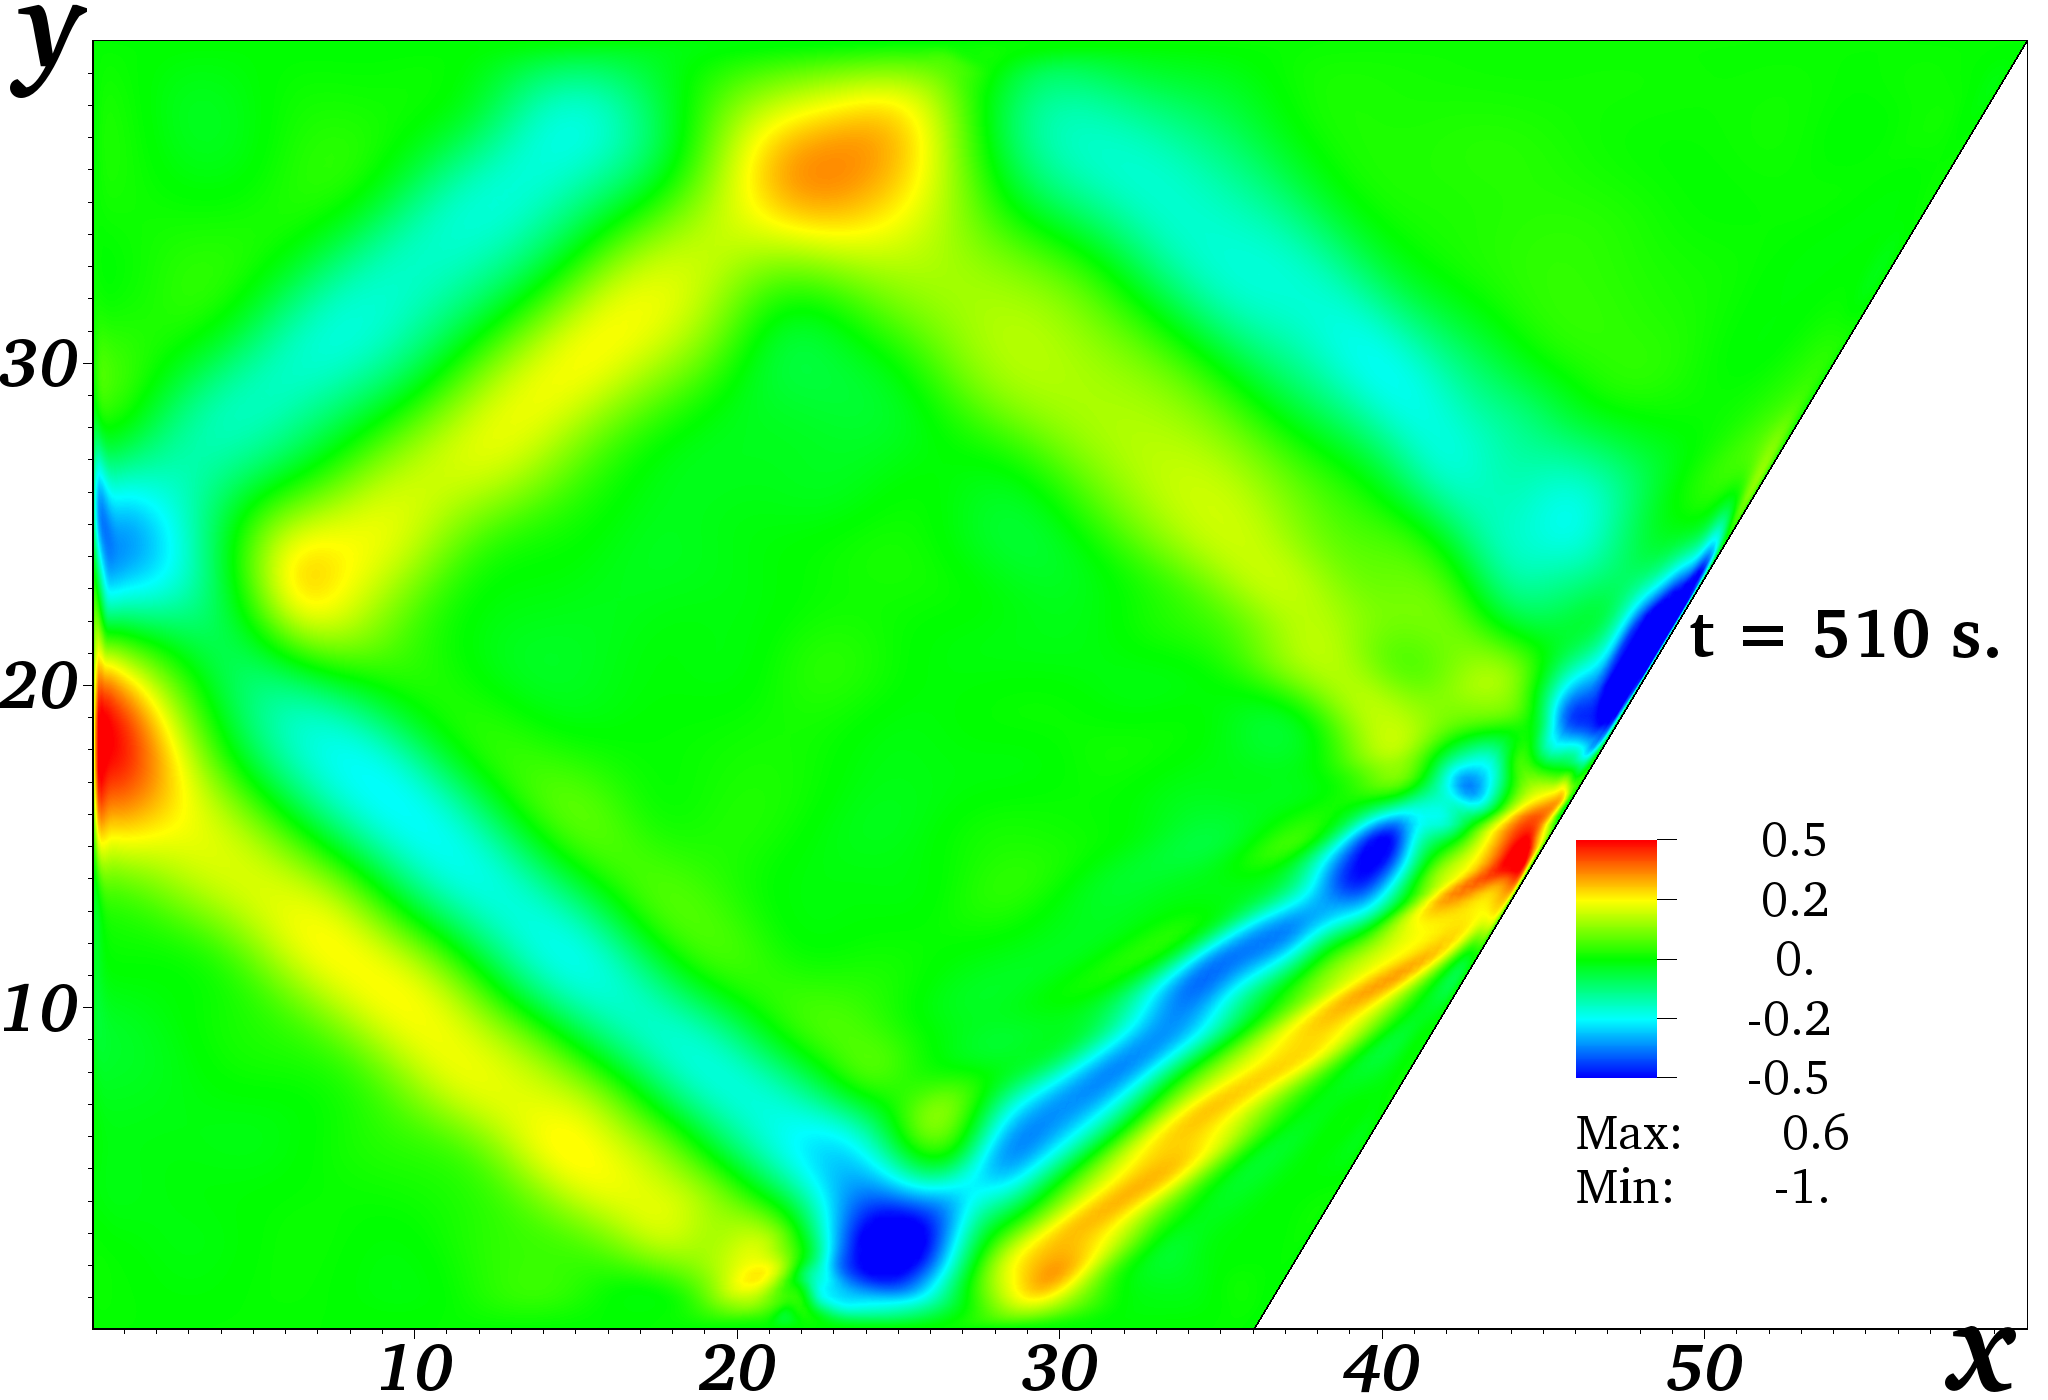
\includegraphics[width=1\textwidth]{../pics/H40L60N1ap05dp20w1p63Deltawp05Biharm/2D36x36DiagramH40L60N1ap05dp20w0p63Deltawp3315BiharmVyn01019.png}
    \caption{Вертикальная компонента скорости при формировании аттрактора}
  \end{subfigure}
  \begin{subfigure}[с]{0.45\textwidth}
    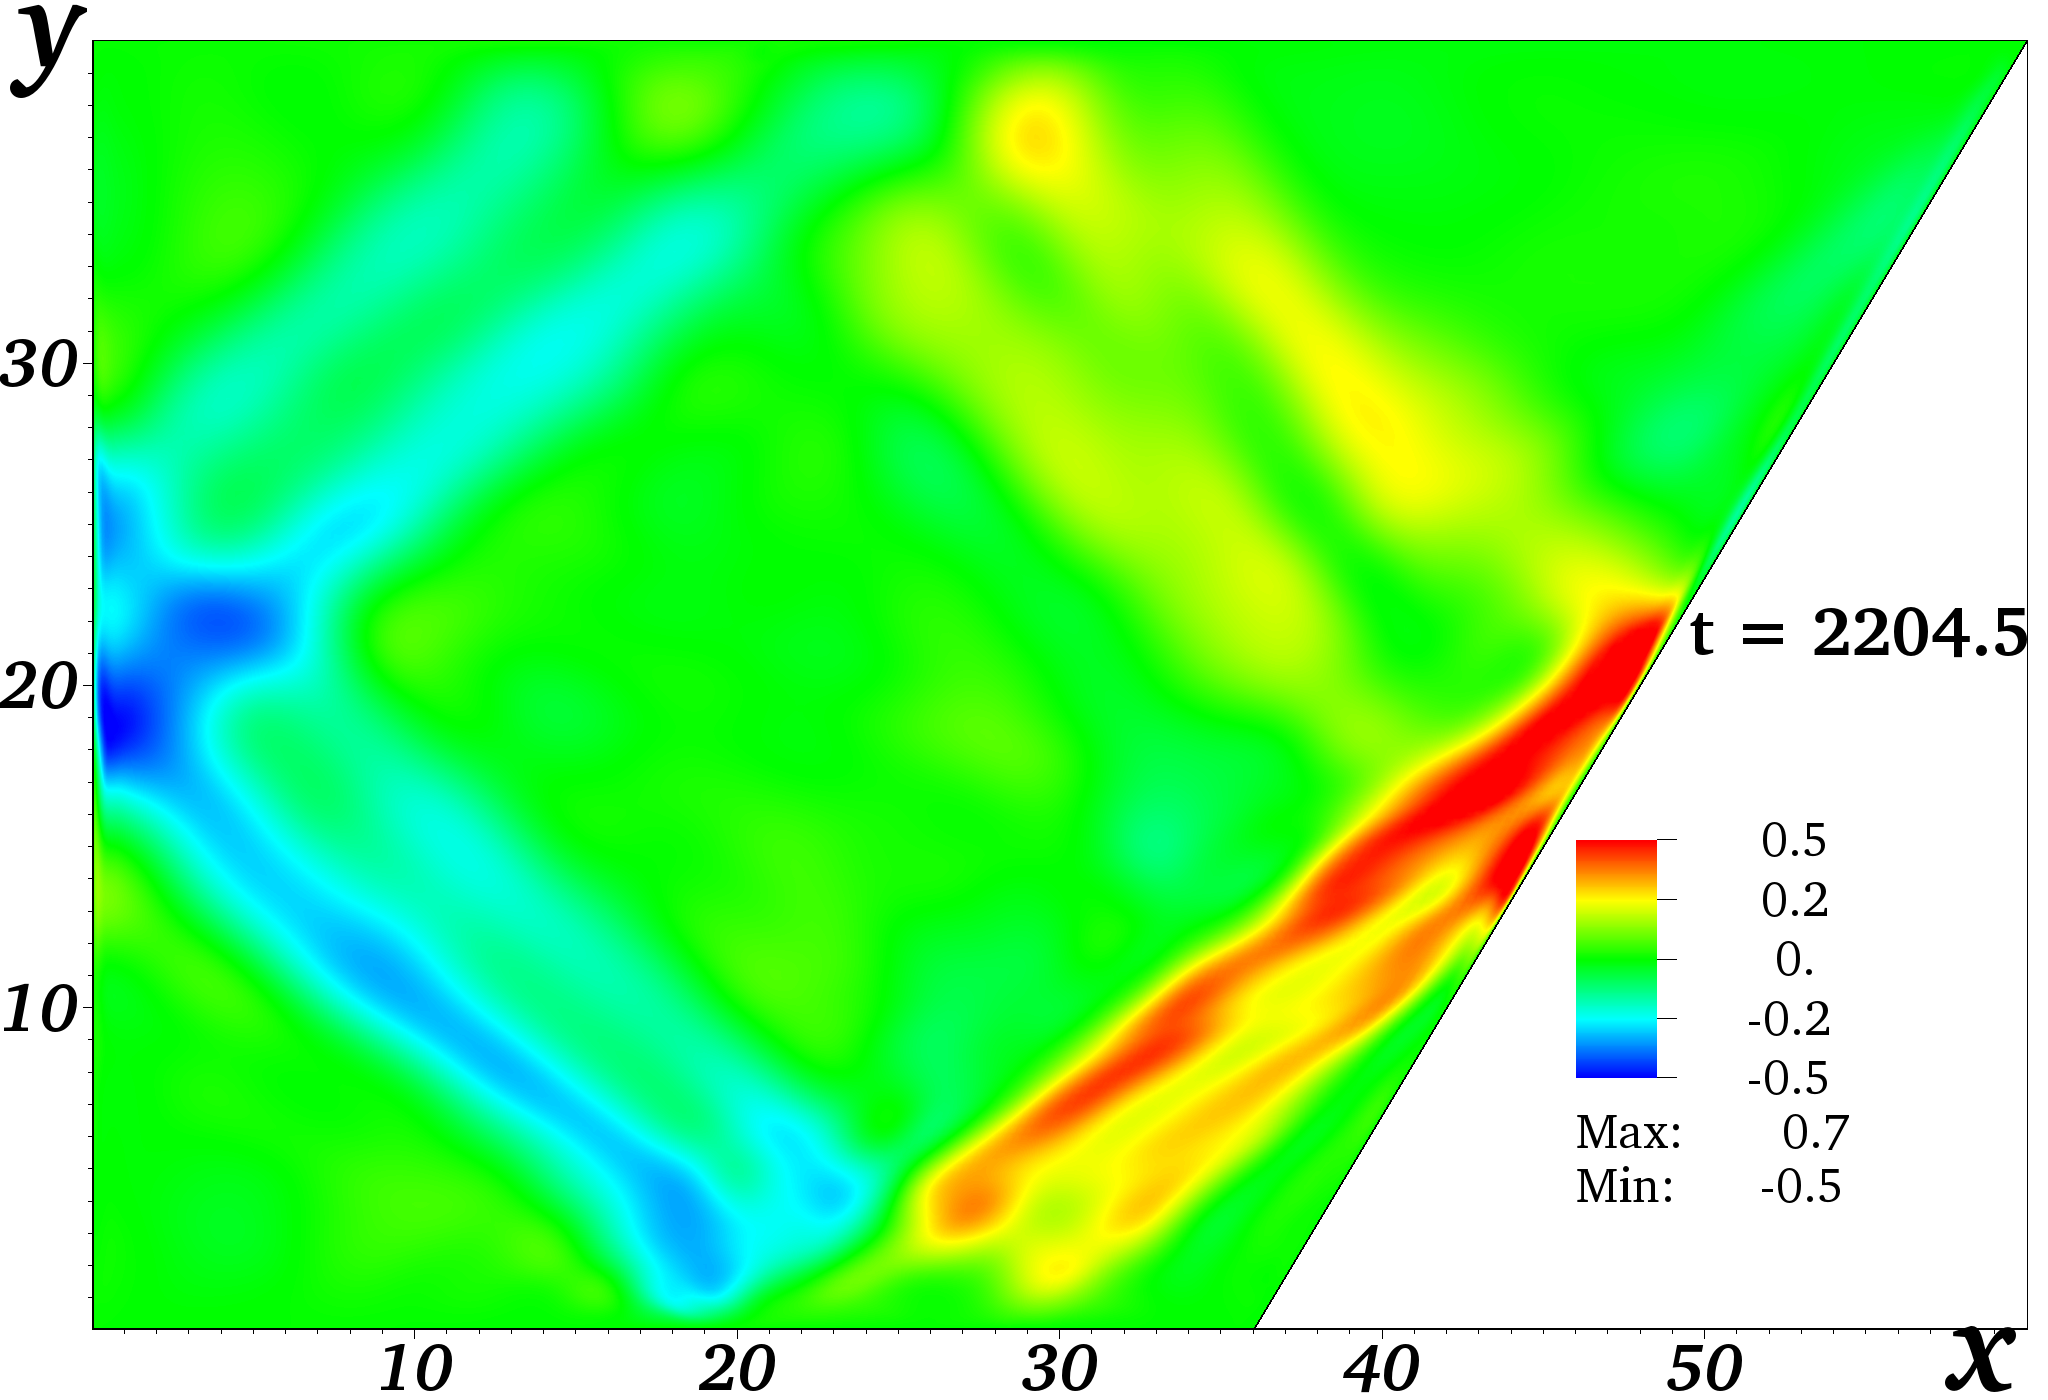
\includegraphics[width=1\textwidth]{../pics/H40L60N1ap05dp20w1p63Deltawp05Biharm/2D36x36DiagramH40L60N1ap05dp20w0p63Deltawp3315BiharmVyn04408.png}
    \caption{Вертикальная компонента скорости при установлении аттрактора}
  \end{subfigure}
  \par
  \begin{subfigure}[с]{0.45\textwidth}
    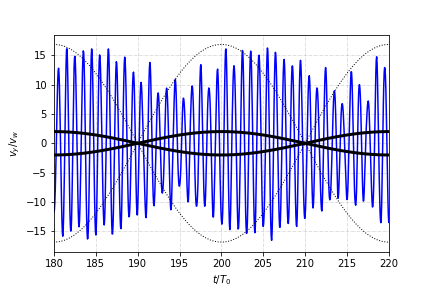
\includegraphics[width=1\textwidth]{../pics/H40L60N1ap05dp20w1p63Deltawp05Biharm/vyX35p57Y11p27t4412.png}
    \caption{Вертикальная скорость}
  \end{subfigure}
  \begin{subfigure}[с]{0.45\textwidth}
    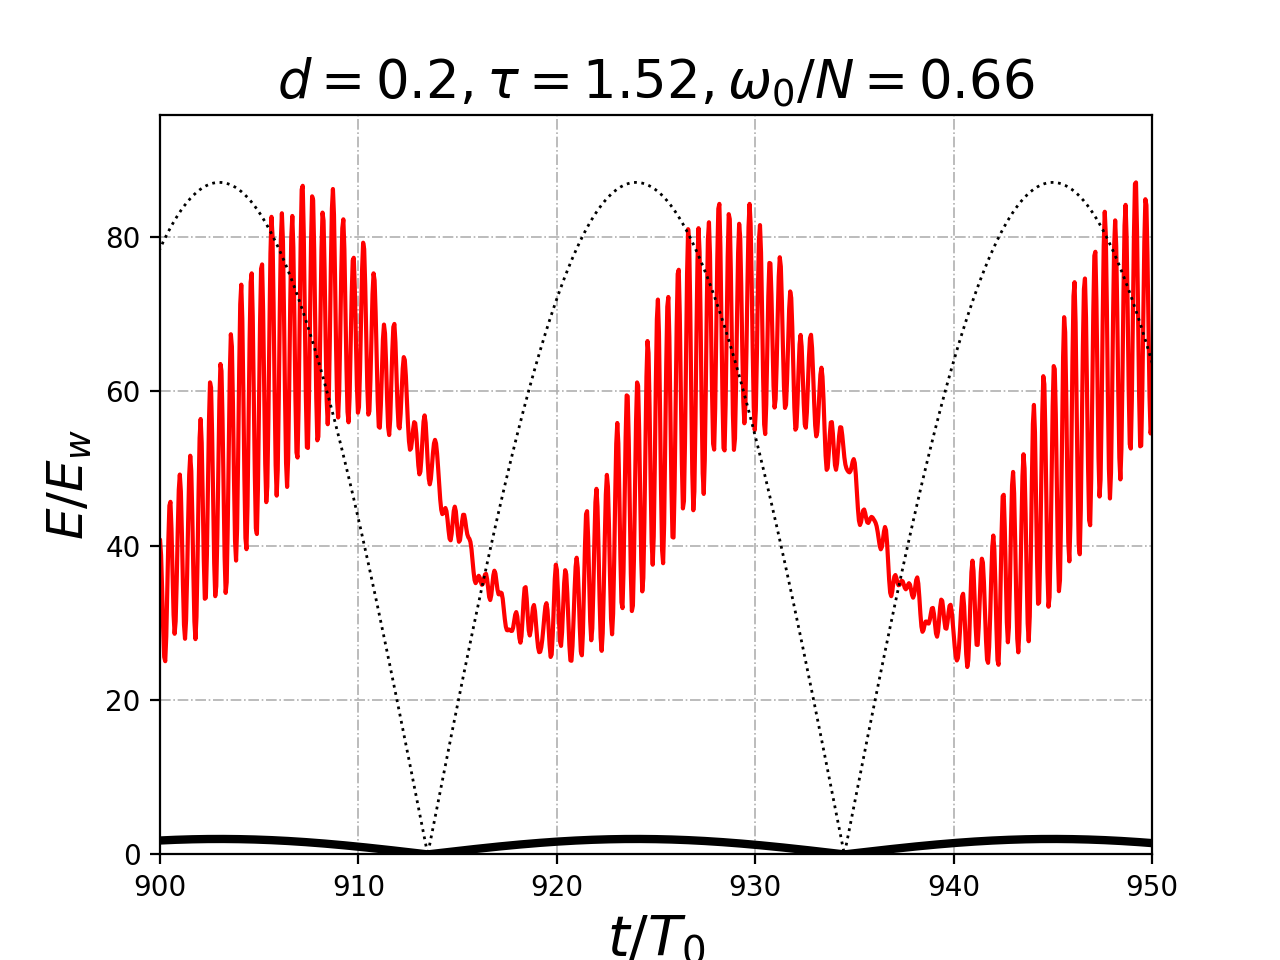
\includegraphics[width=1\textwidth]{../pics/H40L60N1ap05dp20w1p63Deltawp05Biharm/2D36x36DiagramH40L60N1ap05dp20w1p63Deltawp05BiharmtotKEnonDim.png}
    \caption{Кинетическая энергия}
  \end{subfigure}
  \par
  \begin{subfigure}[с]{0.45\textwidth}
    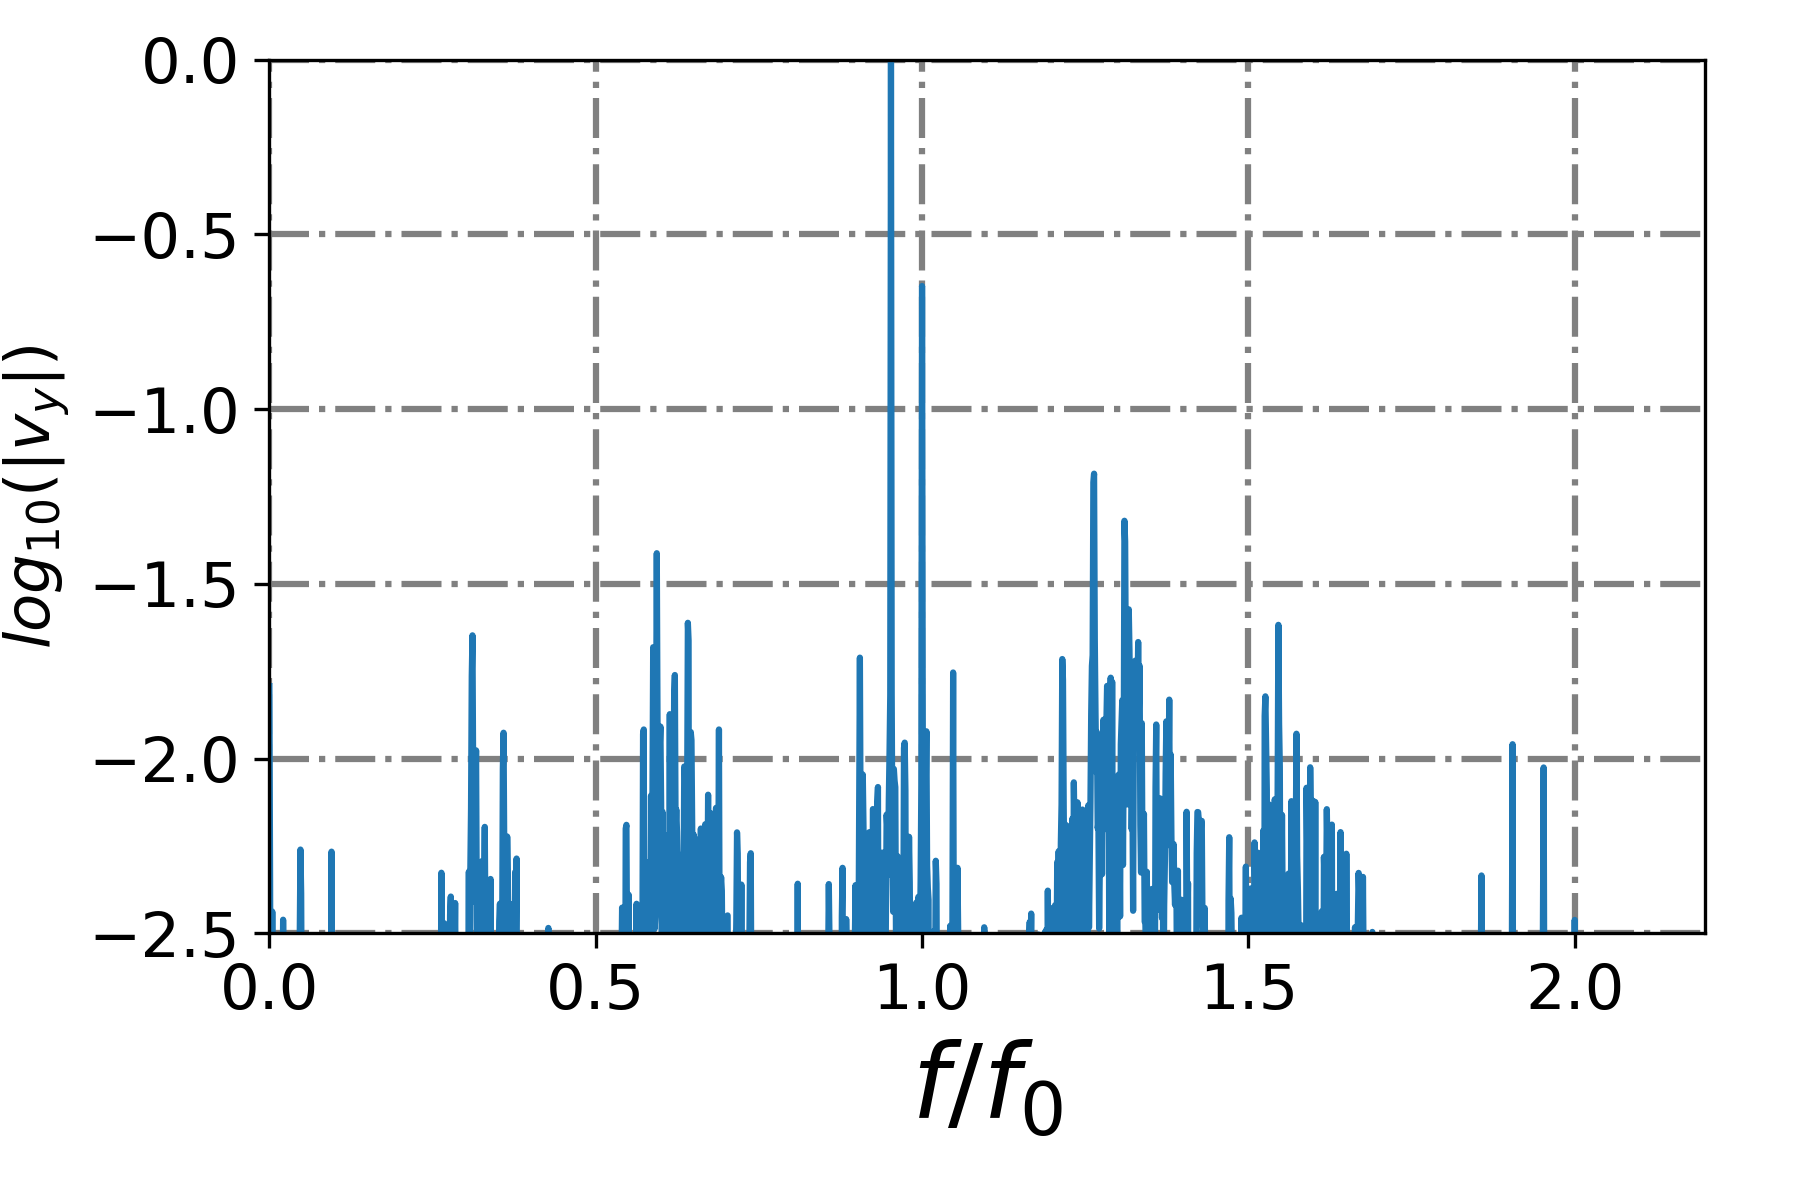
\includegraphics[width=1\textwidth]{../pics/H40L60N1ap05dp20w1p63Deltawp05Biharm/spectrumX35p6Y11p2.png}
    \caption{Спектр}
  \end{subfigure}
  \begin{subfigure}[с]{0.45\textwidth}
    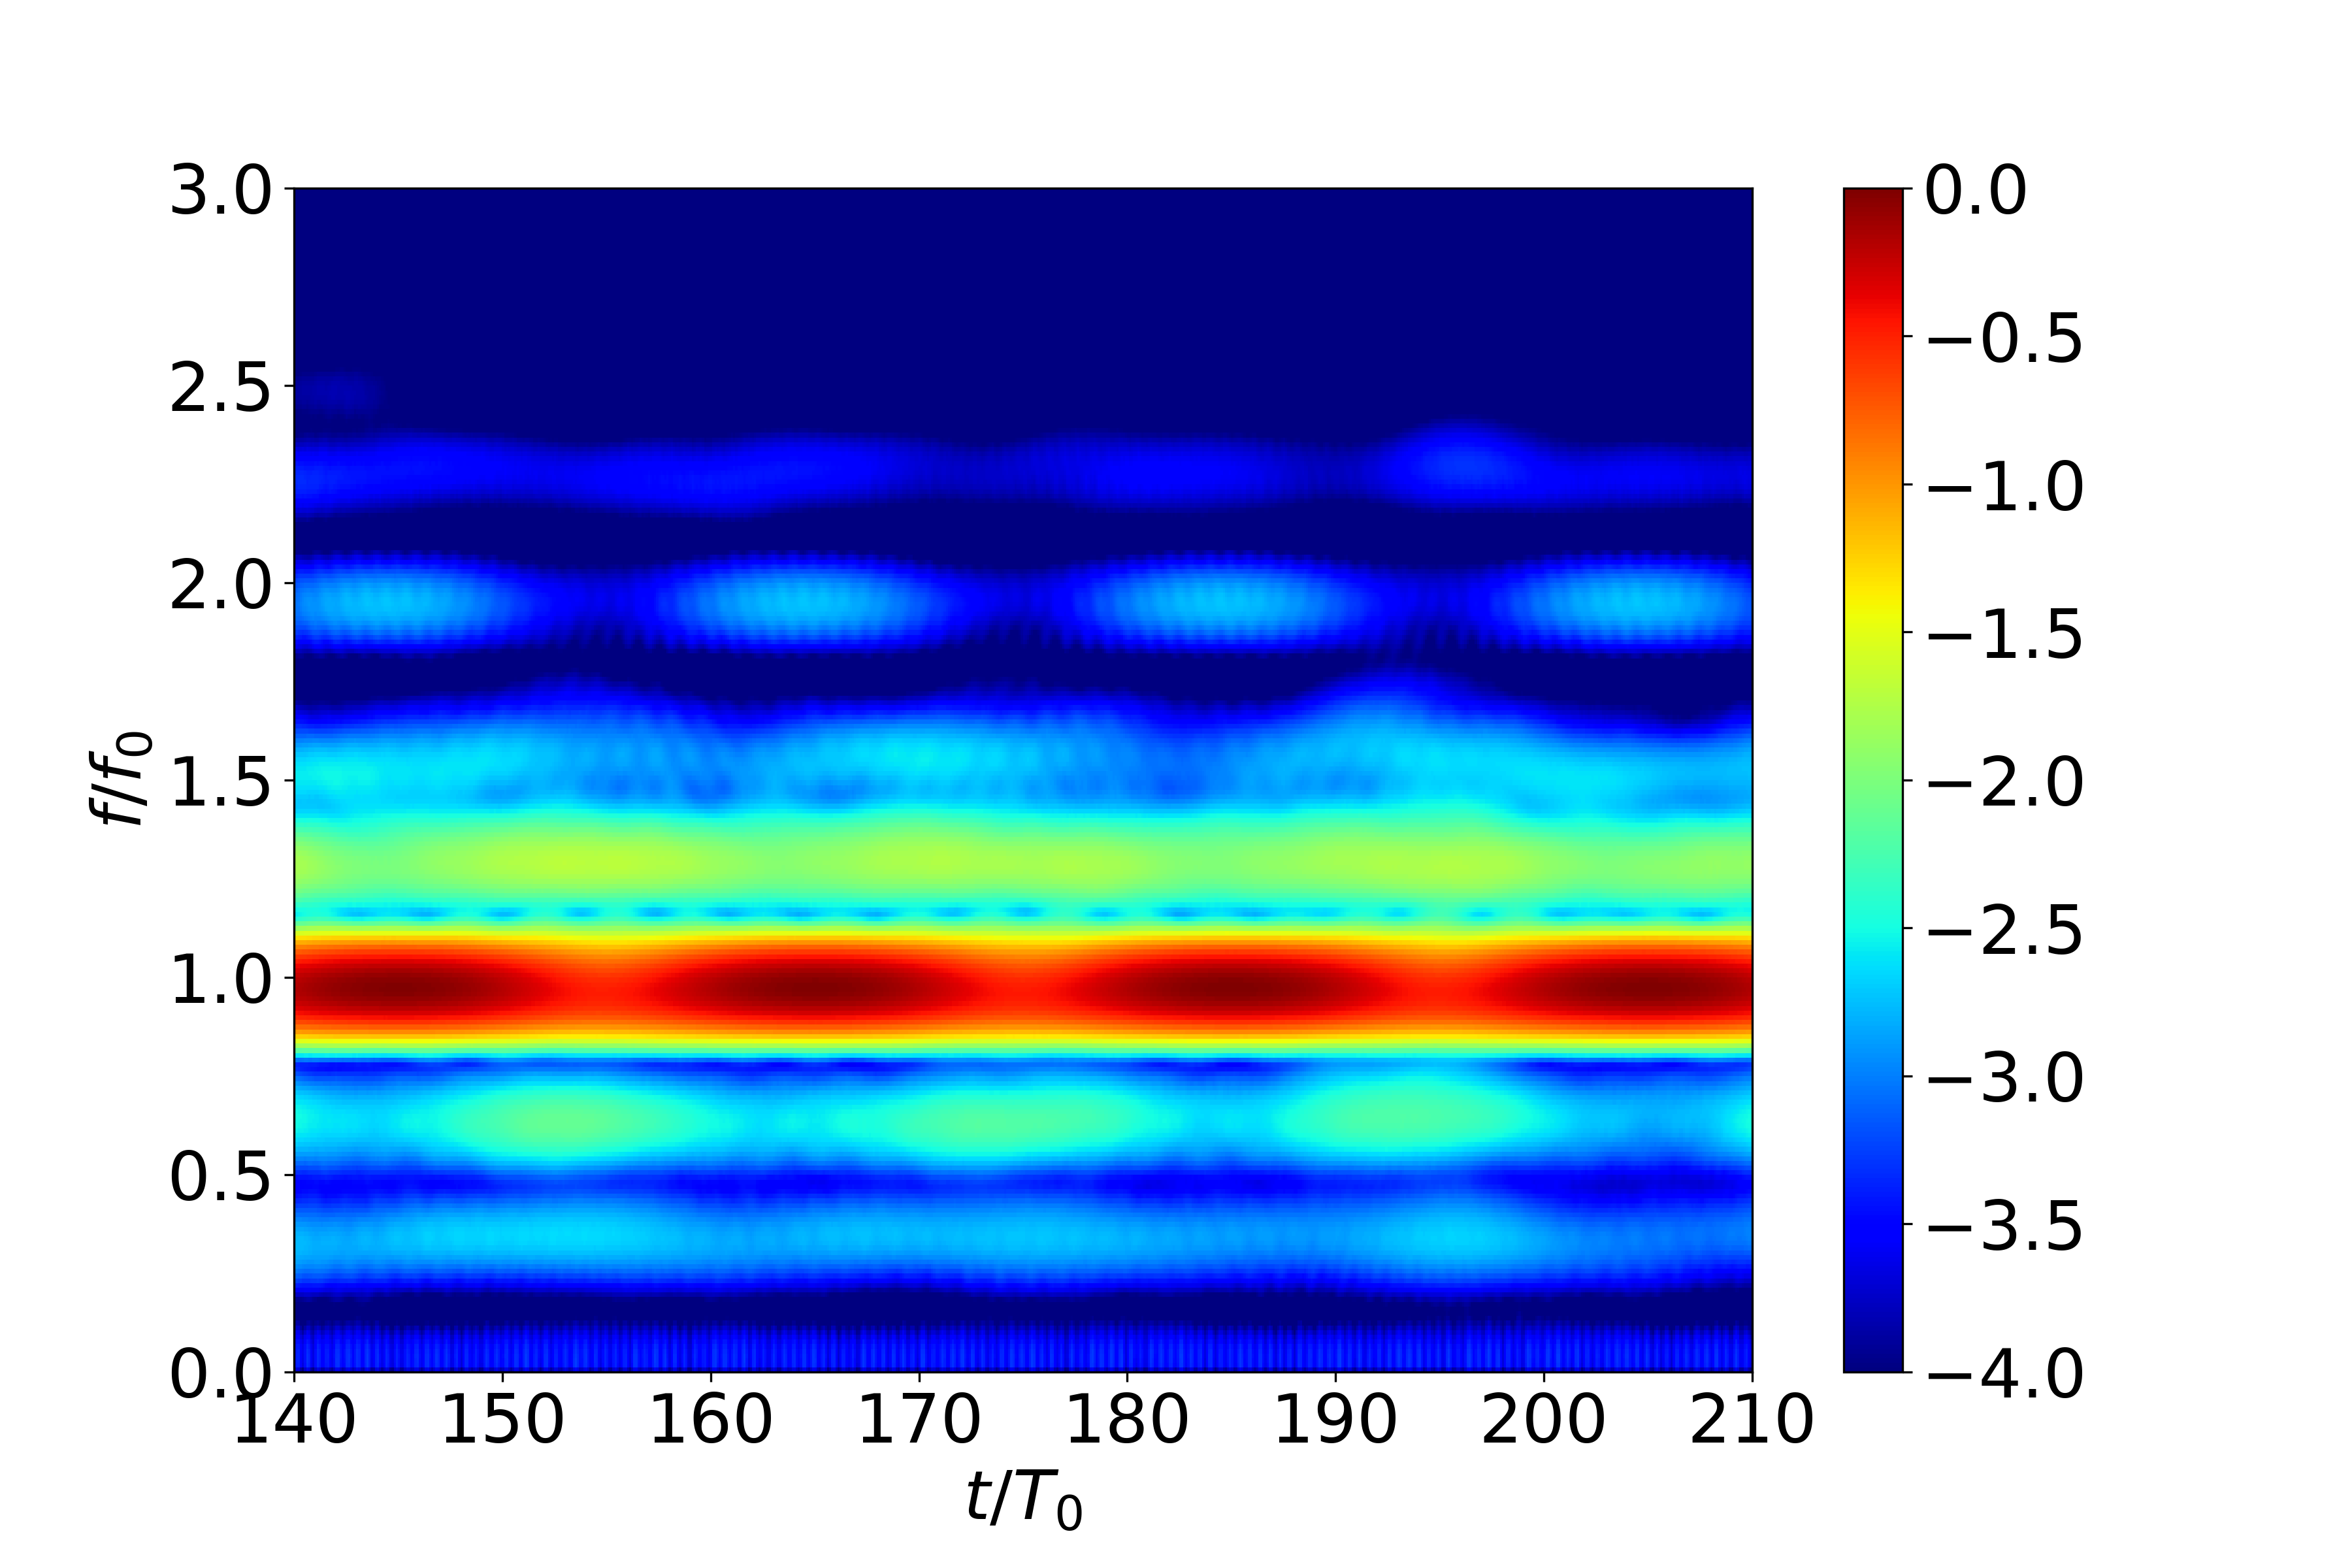
\includegraphics[width=1\textwidth]{../pics/H40L60N1ap05dp20w1p63Deltawp05Biharm/TFspectrumX35p6Y11p2N200.png}
    \caption{Частотно-временная диаграмма}
    \label{}
  \end{subfigure}
  \caption{Результаты количественного исследования характеристик течения стратифицированной жидкости в трапециевидном резервуаре при внешнем воздействии с двумя приближенными частотами $\omega_1/N=0.66$ $\omega_2/N=0.68$. Черной линией  на графиках вертикальной скорости и кинетической энергии показана огибающая амплитуды колебаний волнпородуктора.}
  \label{fig:biharmVyap005-1}
\end{figure}

Выводы диссертационного исследования сформулированные в \textbf{заключении}.

\blfootnote{
\begin{centering}
    Подписано в печать 12.07.2021. Формат 60х84/16.  Усл. печ. л. 0,9. Тираж 60 экз. Заказ А-3. ИПМ им. М.В. Келдыша РАН. 125047, Москва, Миусская пл., 4
\end{centering}
}

\section*{Публикации автора по теме диссертации}
\footnotesize{
\begin{enumerate}[1.]
  \item Бигармонические аттракторы внутренних гравитационных волн / Д. А. Рязанов, М. И. Провидухина, И. Н. Сибгатуллин, Е. В. Ерманюк // \textit{Механика жидкости и газа}  — 2021. — № 3. 
  \item Numerical simulation of three-dimensional wave attractors / I. N. Sibgatullin, E. V. Ermanyuk, K. A. Vatutin, D.A. Ryazanov // \textit{The XXVII workshop of the Council of nonlinear dynamics of the Russian Academy of Sciences.} — 2019. — Vol. 47, no. 1. — P. 112–115.
  \item Numerical simulation of internal wave attractors in horizontally elongated domains with sloping boundaries / I. Sibgatullin, X. Xiulin, E. Ermanuyk, D.A. Ryazanov // \textit{GISTAM 2019 5th International Conference on Geographical Information Systems Theory, Applications and Management.} — SCITEPRESS Heraklion, Crete, Greece, 2019. — P. 366–370.
  \item Openfoam solver based on regularized hydrodynamic equations for high performance computing / M. V. Shatskiy, D. A. Ryazanov, K. A. Vatutin et al. //\textit{2019 Ivannikov Memorial Workshop (IVMEM)} / Ed. by С. П. Прохоров. — IEEE, 2019.
  \item  Численное моделирование трехмерных волновых аттракторов / И. Н. Сибгатуллин, Е. В. Ерманюк, К. А. Ватутин, Д. А. Рязанов, С. Сюй //\textit{Океанология.} — 2019. — Т. 47, № 1.
  \item Openfoam high performance computing solver for simulation of internal wave attractors in stratified flows using regularized hydrodynamic equations / M. Kraposhin, D. Ryazanov, T. Elizarova et al. //\textit{Proceedings of the 2018 Ivannikov ISPRAS Open Conference (ISPRAS, 22-23 Nov. 2018).} — IEEE Xplore Digital Library. — United States: United States, 2018.
  \item Development of openfoam solver for compressible viscous flows simulation using quasi-gas dynamic equations / M. V. Kraposhin, D. A. Ryazanov, E. V. Smirnova et al. // \textit{2017 Ivannikov ISPRAS Open Conference (ISPRAS).} — Vol. 1. — United States: United States, 2017.
  \item Numerical simulation of compressible gas flows using regularized gas dynamic equations solver qgdfoam / M. V. Kraposhin, T. G. Elizarova, M. A. Istomina et al. // \textit{AIP Conference Proceedings 1959}, 030013 (2018). — Author(s), 2018.
\end{enumerate}
}
\end{document}